\documentclass[a4paper]{article}
%Commented in draft to allow for notes.
\usepackage{fullpage}
\usepackage{hyperref}
\usepackage{todonotes}
\usepackage{censor}
\setlength\parindent{0pt}

\title{Robotic Swarms: \\Distributed Coordination Without Location}
\author{S.J.A. Bekhoven  \and
    S.P. Metman \and
    M.J. Rogalla}
\date{\today}

\pagestyle{empty}

\begin{document}
\maketitle
\thispagestyle{empty}

\begin{abstract}
This is the abstract of my paper.
This is the abstract of my paper.
This is the abstract of my paper.
This is the abstract of my paper.
This is the abstract of my paper.
This is the abstract of my paper.
This is the abstract of my paper.
This is the abstract of my paper.
This is the abstract of my paper.
This is the abstract of my paper.
This is the abstract of my paper.
This is the abstract of my paper.
\end{abstract}

% Do not compile individual files, compile only this main file.

\section{Introduction}
  %!TEX root = ../Bachelorseminar-RoboticSwarms.tex

Swarm robotics has become a prominent and promising research area in the recent years. 
It has great potential use for a large variety of applications, some of which have already been successfully implemented. 
We want to provide a global overview of the main problems found in the research area of robotic swarms. 
Many articles already exist which give an overview of applications and used practices in this area, but often do not explain the problems underlying these practices. 
Therefore, we focus on providing a problem-oriented overview of the robotic swarms, while also providing a general overview of best practices and solutions of these problems.\\
\\
We start by defining some terminology, since some of the terms used in robotic swarms are ambiguous and can be interpreted in different ways.
We define a swarm as a scalable network of robots which consists out of more than two robots.
Furthermore, we only consider robotic swarms in which every robot has some form of distributed intelligence.
An exception is of course when a swarm of multiple robots is controlled by one control station.
Because the swarm robots have to communicate either directly or indirectly with each other, the swarm will still have some form of distributed intelligence to function.
% Thus, according to our original definition, we still regard it as a swarm. \\
\\
\\
Robotic swarm algorithms can roughly be characterized by their location type and their information type. Algorithms can then respectively be either \emph{location-based} or \emph{location-free} and either \emph{range-based} or \emph{range-free}:
\begin{description}
	\item[Location-free] Robots have no knowledge and do not keep track of their absolute or relative location.
	%A robotic swarm is \emph{location-free} if the swarm has no knowledge of the boundaries of the location it is in, whether it is provided at the beginning or is actively searched for during the execution of the algorithm. 
	\item[Location-based] Robots have perfect knowledge or keep track of their absolute or relative location.
	%A robotic swarm is \emph{location-based} if each individual robot in the swarm has the knowledge of its absolute or relative location.
	\item[Range-free] Robots do not communicate or communicate via some kind of central base.
	%A robotic swarm is \emph{range-free} if each robot can detect the presence of other nearby robots or obstacles, but does not store or measure the distance towards the other object.
	\item[Range-based] Robots communicate within predetermined range.
	%A robotic swarm is \emph{range-based} if each robot in the swarm keeps track of the exact distance between itself and the other robots in the swarm or obstacles. 
\end{description}

In the following sections, we compare the algorithms by two characteristics. 
The first characteristic is \emph{scalability}, by which we mean the ability of maintaining performance when the population in the robot swarm is increased. 
The second is \emph{performance}, by which we mean the general efficiency. 
We define efficiency separately for each problem before comparing the algorithms of that problem. 
We do this because the solutions have different ways of expressing efficiency for each problem.\\

A composite problem is a problem composed of multiple main problems in such a way that these main problems influence the working of the solutions. 
Although such a composite problem can be singled out, a lot of the main problems have some form of overlap too, although not with significant impact. 
The main problems Dispersion and Source Localization both include the Formation problem, and the Collective Transport is composed of the Formation problem among others.
The Exploration problem is more of an extension to the Dispersion problem. 
This relationship is shown in the Figure~\ref{fig:ProblemsOverview} \\
\begin{figure*}
  \centering
  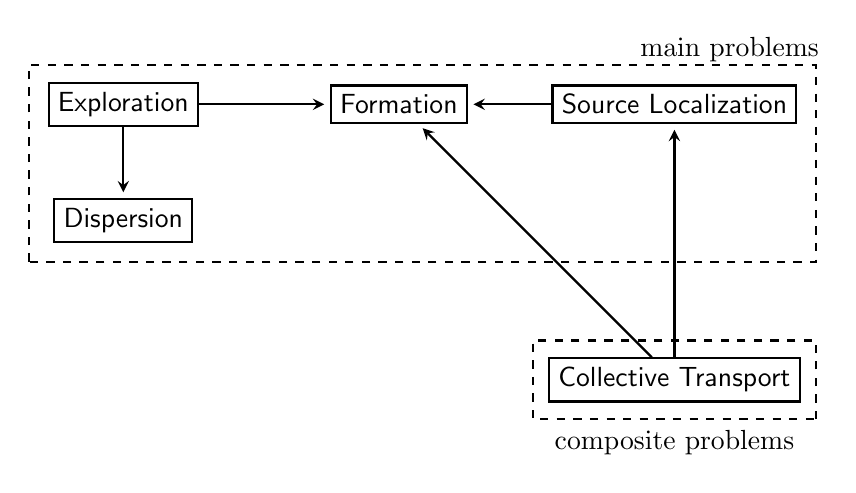
\begin{tikzpicture}[->,>=stealth,shorten >=2pt,auto,node distance=3.5cm,
    thick,main node/.style={fill=white,draw,font=\sffamily}]
    \node at (7.7,0.7) {main problems};
    \node at (7,-4.3) {composite problems};
    \draw[fill=white,dashed] (-1.2,-2) rectangle (8.8,0.5);
    \draw[fill=white,dashed] (8.8,-4) rectangle (5.2,-3);
    \node[main node] (1) {Exploration};
    \node[main node] (2) [below= 0.9cm of 1] {Dispersion};
    \node[main node] (3) [right of=1] {Formation};
    \node[main node] (4) [right of=3] {Source Localization};
    \node[main node] (5) [below of=4] {Collective Transport};

    \path[every node/.style={font=\sffamily\small}]
      (1) edge [right] node[left] {} (2)
      (4) edge [right] node[left] {} (3)
      (5) edge [right] node[left] {} (4)
      (5) edge [right] node[left] {} (3)
      (1) edge [right] node[left] {} (3);
  \end{tikzpicture}
  \caption{Problem Composition Overview} \label{fig:ProblemsOverview}
\end{figure*}



The remainder of this paper is then structured as follows. 
In Section~\ref{sec:Formation} until Section~\ref{sec:Localization} we define the main problems in robotic swarms. 
Then, in Section~\ref{sec:CollectiveTransport}, we discuss the composite problem Collective Transport. 
For each problem we mention the possible real-life applications, their subproblems and the underlying algorithms of the solutions.
After that we discuss the characteristics of each algorithm, the corresponding (dis)advantages and where possible some remaining problems.
For more information on the operation of the mentioned algorithms, you can check the references provided. 
Finally we briefly discuss our observations in Section~\ref{sec:Discussion}.





\section{Definitions from Literature}
  %!TEX root = ../Bachelorseminar-RoboticSwarms.tex
This section will provide some definitions so that there will exist no ambiguity for some terms. Firstly, we wish to define what robotic swarms are. A robotic swarm is a collection of robots. In this review, we will only consider something a swarm when the amount of robots is higher than two and the amount can be scalable; so a swarm of only two robots that doesn't interact with a third robot will not count as a swarm.  \\
Furthermore, in this review we will only consider robotic swarms in which each robot is not controlled individually; they should have some form of distributed intelligence. An exception is of course when a swarm of multiple robots is controlled by one control station; this swarm will still have some form of distributed intelligence to function and thus is considered a swarm.  \\

Robotic swarm applications can roughly be characterised by two attributes; they are either \emph{location-based} or \emph{location-free}, or they are either \emph{range-based} and  \emph{range-free}. A location-free approach does not exclude a range-free approach and vice-versa; they are two different ways of approaching an application. The definitions of these attributes may be interpreted ambiguously, which is why we will define it here. The definitions are:

  \begin{itemize}
    \item A robotic swarm is \emph{location-free} if the swarm has no knowledge of the boundaries of te location it is in, whether it is provided at the beginning or is actively searched for during the execution of the algorithm. 
    \item A robotic swarm is \emph{location-based} if the swarm has the knowledge of predefined boundaries of the location it operates in, whether provided at the beginning of the execution of the algorithm or if it is actively searched for. 
    \item A robotic swarm is \emph{range-free} if each robot can detect the presence of other nearby robots or obstactles, but does not store or measure the distance towards the other object.
    \item A robotic swarm is \emph{range-based} if each robot in the swarm keeps track of the exact distance between itself and the other robots in the swarm or obstacles. 
  \end{itemize}

  
\section{Applications}
  %!TEX root = ../Bachelorseminar-RoboticSwarms.tex
Robotic swarms can be used for many real-world applications as for example in tasks that cover a region, tasks that are to dangerous for human beings, tasks that scale-up or scale-down in time or tasks that require redundancy \cite{csahin2005swarm}. In this chapter, we will name a few of the most-used techniques used by actual applications of robotic swarms, and give examples of applications that use these techniques.

  \subsection{Exploration}
  %!TEX root = ../Bachelorseminar-RoboticSwarms.tex
Exploration is a technique in which a swarm of robots try to fully explore an environment, which is one of the fundamental problems faced in mobile robotics. 
The main goal is to minimize the overall exploration time while still exploring the whole environment. 
The main problem faced when trying to achieve this goal is finding appropriate target points for each individual robot so that they simultaneously explore different regions of the environment. \cite{burgard2005coordinated} \\
The exploration technique is found in many robotic swarms techniques, for example in \emph{path-finding}, \emph{collective transport} and \emph{surveillance}.
Practical applications that apply the exploration technique are for example rescue missions. \cite{Naghsh2008,Penders2011}
In this particular paper, a robotic swarm applying the exploration technique is used to assist navigation for firefighters, used in situations in which their vision is blocked by smoke and obstacles. 
A last example of an application is cleaning. \cite{wagner2008cooperative}
Here, the exploration technique is used to clean a surface with cleaning robots, that communicate in a swarm, as fast and as efficient as possible. 
Of course, exploration techniques are used in many more different robotic swarm applications, and is the building block for many different other techniques. 

%Exploring an environment is one of the fundamental problems faced in mobile robotics. 
%The main goal is to minimize the overall exploration time and the main problem faced when trying to achieve this goal is finding appropriate target points for each individual robot so that they simultaneously explore different regions of the area \cite{burgard2005coordinated}. 
%Robotic swarm exploration can be used for real-world applications like rescue missions \cite{Naghsh2008,Penders2011}, surveillance \cite{Burkle2010} and cleaning \cite{wagner2008cooperative}.
  
  \subsection{Mapping}
  %!TEX root = ../../Bachelorseminar-RoboticSwarms.tex

Mapping is a technique in which a swarm of robots try to make a map of the surrounding unknown environment. 
The mapping of an unkown environment can be efficiently done with the usage of robotic swarms; this is called collaborative mapping. 
As with other algorithms, this mapping should be done as fast as possible without losing accuracy. 
The core of the mapping technique looks very similar to exploration, but an important difference is that in mapping a map should be made and stored. 
This leads to more communication between robots and more distributed intelligence. \\

Mapping of an unknown environment is very useful in hazardous and unaccessable environments. \cite{hardin2004modified}
In this paper a practical application is mentioned, the detection of hazardous aerosol in a contaminated, confined area. 
Robotic swarms are used in this work because it is safer to use them. 
Of course, as mentioned earlier, some techniques overlap, and mapping is no exception to this. 
The mapping technique uses elements of exploration, dispersion and localization.  

%OLD
%The mapping of an unkown environment can be conveniently done with the usage of robotic swarms, this is called collaborative mapping. 
%Collaborative mapping is very useful in hazourous and unaccessable environments.\cite{hardin2004modified} 
In \cite{sheng2006distributed} a model is described in which the robots have limited communication range and full knowledge of their location. By continuously looking for the closest undiscovered area in combination with a nearest measure it tends to explore the complete area by staying together and continiously updating each others maps.
Some of the techniques used in these types of applications are localization, exploration, dispersion, mapping. \cite{sheng2006distributed,rothermich2005distributed} 
  
  \subsection{Dispersion}
 %!TEX root = ../Bachelorseminar-RoboticSwarms.tex

  \emph{Swarm-Assisted Exploration makes interactive use of autonomous robots in exploration settings. The swarms of robots are capable of supporting and enhancing operations co-operatively with each other and are coordinated by a single human supervisor.}\cite{Naghsh2008,Penders2011}
    The techniques required for Swarm-Assisted Exploration include, but are not limited to: \emph{foraging}, \emph{formation}, \emph{mapping} and \emph{exploration}.\cite{Naghsh2008,Penders2011} The foraging techniques are needed in order to give the swarm the ability to search and locate subjects. Formation is required in order for the swarm to navigate optimally and prevent conflicts in exploration. The mapping and exploration service are required to create a well constructed map of the explored area, such that the human and other robots are aware of their surroundings, even if it is impossible to get a visual due to reduced visibility.

  \subsection{Localization}
 %!TEX root = ../Bachelorseminar-RoboticSwarms.tex

  \emph{Due to the ambiguity of this name, there have been many applications which have aimed to achieve this, from nuclear spills and oil spills to fire-origins. Much of this however is theoretical work, due to the fact that the price of these individual robots is still rather high.}

  Some of the techniques used in toxic source discovery are: control, communication and distribution.\cite{Li2012}

 \subsection{Path-finding}
 %!TEX root = ../../Bachelorseminar-RoboticSwarms.tex

  Path finding or path planning (in this paper we will use path finding) basically is the basis of every robotic swarm technique, since every distributed algorithm in mobile robotics tries to find the best location to go to from its current location. In this paper we consider path finding as the problem to find the optimal collision free path from the start state to the goal state. \cite{qin2004path}. Path finding can be used in multiple real-life applications such as foraging (trying to find food sources and bring food back to the basis) \cite{hoff2010two} and searching (for spills, victims, targets) \cite{pugh2007inspiring} and is often combined with some form of particle swarm optimization \cite{poli2007particle}.

\subsection{Collective transport}
%!TEX root = ../../Bachelorseminar-RoboticSwarms.tex

Collective transport of objects is the technique of a swarm of robots locating an object and collectively moving the object to another place, like a homebase. 
This can be compared to a foraging technique; although this implies that a path is made to a certain place. 
This does not apply to all collective transport techniques. \cite{hoff2010two}  
It can be easily seen that localization is an important part of the collective transport technique, and thus has much overlap .\\
Transporting objects by robotic swarms has many potential applications in many settings, from agriculture to construction to disaster relief. 
Especially in dangerous settings like warzones or radio-active areas, robotic swarms can be a powerful tool to safely retrieve many objects. 
More so because the robots used for this application are cheap to produce. 


%For this application to work, each agent only has to know the target direction but does not have to know the object shape, weight, its own position or the position and number of other agents. This makes this application location-free and range-free. An extra invariant is that there must be enough robots to overcome the static friction of the object to be transported.  \cite{Rubenstein}


\subsection{Surveillance}
%!TEX root = ../Bachelorseminar-RoboticSwarms.tex

Surveillance is a technique in which a swarm of robots continuously patrol the same space, and simultaneously keep an eye out for abnormalities which are specified beforehand. Often this technique also includes formation, because patrolling robots should be in the same formation. Furthermore, in unknown locations mapping would be used, and in locating abnormalities a localization technique is often used. \\
Surveillance with a single robot is already a powerful tool, but with a swarm of robots it becomes even more effective. A larger area can be covered, local communication can be handled efficiently and depleted robots can interchanged with other robots. The applications of swarm surveillance are diverse, and are already used in a vast range of applications like agricultural practices, police surveillance, inspecting unreachable locations, patrol missions and reconnaisance tasks. \cite{Burkle2010} \\
The application can be implemented in many different ways, but is able to work location-free and range-free, but in some applications the location is already known and in others it can be helpful for a robot to know the exact location of the other robots of the swarm. In some applications the process isn't even completely autonomous; a human user could be in a ground control station. Some of the techniques used in swarm surveillance are: dispersion, localization, distributed communication and exploration. 

\subsection{Formation}
%!TEX root = ../Bachelorseminar-RoboticSwarms.tex

  \subsection{Exploration}
  \textbf{Description: }\emph{Cleaning/exploring a component in an unkown area is a common problem which can be solved effectively by using a tobotic swarm. For example in \cite{wagner2008cooperative} a swarm of robots is placed in a certain component which has to be cleaned totally. The robots have limited visibility and can only see other robots within a certain distance. Main goal is to not disconnect the component that has to be cleaned to be sure that the component will be get fully cleaned in the end.} \\
  The main techniques that are described in \cite{wagner2008cooperative} are algorithms that preserve the connectivity of the spot to be cleaned and prevent the clustering of robots.




  
  \subsection{Overview}
  Give an overview of real-world applications possible with Robotic Swarms. A list of possible applications:
    \begin{enumerate}
      \item Area Cleaning
      \item Space Exploration (swarm of Mars rovers)
      \item Rescue Missions
      \item Treacherous Radioactive Survey
      \item Survey and cleanup of Toxic Spills
      \item Surveillance
      \item Swarm-Assisted Fire Fighting
     \item Collective Transport of Complex Objects
    \end{enumerate}
  \textbf{Categories}
    \begin{itemize}
      \item Region Covering
      \item Dangers
      \item Scaling in time
      \item Redundancy
    \end{itemize}
  
 
 \section{In-depth review of Techniques}
  %!TEX root = ../Bachelorseminar-RoboticSwarms.tex
A small introduction to the section\ldots
    \subsection{Communication}
    \input{./tex/Techniques/Communication.tex}
    \subsection{Exploration}
    %!TEX root = ../../Bachelorseminar-RoboticSwarms.tex

\subsubsection{Collaborative multi-robot exploration [1]}
\cite{burgard2005coordinated}
Should be divided into Mapping \& Localization which are in my opinion two types of exploration with too much overlap.

    \subsection{Dispersion}
    %!TEX root = ../../Bachelorseminar-RoboticSwarms.tex

One of the key techniques used in robotic swarms is dispersion. The goal of dispersion in the context of robotic swarms is to scatter the individual robots in an environment such that every section of the environment can be covered. In this section we will focus on non-location oriented algorithms. If prior knowledge about the exact location is provided, a formation technique should be used.

\subsubsection{Algorithms}
	The following dispersion algorithms are the most widely used algorithms and thus will be taken into our analysis. A very brief description is given of each algorithm. For more information on the operation of these algorithms, please consult the references.\\

	\textbf{Location-Free Dispersion Algorithms}
	\begin{itemize}
		\item \textbf{Depth-First Leader-Follower Strategy (\emph{DFLF})}\cite{hsiang2004algorithms}:\\
			A \emph{Depth First Search}(DFS) inspired algorithm in which the swarm has one leader at any given point in time. The robotic swarm has the overview of a map in which specific regions, called \emph{pixels}, are defined. \emph{Frontier pixels}, are pixels which haven't been traversed yet. The leader robot keeps looking for frontier pixels until there are none left and stops and tells its \emph{successor robot} to be the leader. If there are no successors left, the algorithm halts and the total dispersion of the area. The other robots always try to follow the leader and traverse the tiles around it.
		\item \textbf{Breadth-First Leader-Follower (\emph{BFLF})}\cite{hsiang2004algorithms}:\\
			A \emph{Breadth First Search}(\emph{BFS}) inspired algorithm, which does not exactly perform \emph{BFS}, but approximates it. It is a more complex algorithm than the \emph{DFLF} algorithm, but has to make fewer moves to fully cover the map. In an extension of the \emph{DFLF} algorithm, the \emph{BFLF} algorithm also contains a waiting state, in which a robot pauses to make the next move. Furthermore, instead of having only one leader, this algorithm allows for multiple leaders. The leaders again strive to find all the frontier pixels, but now also make sure that the follower robots don't stray to far away. Once no frontier pixels can be found by the leader, the leader waits for the followers to arrive and passes on its leadership to one of the followers, the successor. The \emph{BFLF} strategy tries to create as many paths as possible. Visited pixels form a tree, the tree can be branched, which then represent the alternate pixels reachable from that pixel. This branching balances the flow by giving the possiblity to go through pixels multiple times, to be able to go into differerent directions.
	\end{itemize}
	\textbf{Range-Based Dispersion Algorithms}
	\begin{itemize}
		\item \textbf{Directed Dispersion/Disperse Uniformly}\cite{mclurkin2007distributed}:\\
			The directed dispersion algorithm has the goal to disperse the robots quickly and uniformly, while keeping the robots connected. The algorithm consists of two sub-algorithms: \emph{disperseUniformly} and \emph{frontierGuidedDispersion}. The \emph{disperseUniformly} algorithm spreads the robots evenly with given constraints. It works by calculating an opposite direction vector of the positions of the nearest robots. This means that communication between robots is of vital importance. The \emph{frontierGuidedDispersion} directs robots towards unexplored areas, while keeping the robots connected. It uses robots which are on the frontiers of explored space to guide the Swarm in unexplored space. An optimal path is created for the other robots to move optimally towards the frontier. For an exact description of the implementation of these algorithms please see \cite{mclurkin2007distributed}.
		\item \textbf{Random Walk}\cite{morlok2007dispersing}:\\
			This algorithm has 2 states: \emph{walking} and \emph{avoid obstacle}. In the \emph{walking} state each robot keeps going straight with an orientation which randomizes over a certain time interval until there is an object and switches to the \emph{avoid obstacle} state. In the case that it detects a possible collision, the robot changes orientation dramatically until the obstacle has been avoided and continues in the \emph{walking} state.
		\item \textbf{Follow Wall}\cite{morlok2007dispersing}:\\
			The follow wall algorithm has 4 states: \emph{find wall}, \emph{align to wall}, \emph{follow wall} and \emph{navigate corner}. The details of this algorithm will not be discussed, as there are quite a few major flaws in this algorithm. This algorithm does not take the existance of other robots into account and thus it is possible for robots to see each other as walls. The usage of this algorithm for dispersion is thus very limited and should be avoided.
		\item \textbf{Seek Open}\cite{morlok2007dispersing}:\\
			By calculating an average obstacle vector with support of distance censors, a vector in the exact opposite direction is calculated and the robot, will follow this vector. Depending on the magnitede of the vector, a new assesment will be done once the robot reaches the approximated location. This means that the robot does not need to take further care of collisions with walls, but it is possible for robots to run into each other, or other dynamically moving objects, unless collision avoindance is separetely implemented.
		\item \textbf{Fiducial} \cite{morlok2007dispersing}:\\
			By using a beacon system, every robot is able to get the relative location of other robots within a certain range. This information is the used to steer away from the other robots. If no robots are in range, the robot uses the \emph{Random Walk} algorithm.
		\item \textbf{Clique-Intensity}\cite{ludwig2006robotic}:\\
			This algorithm uses the connectivity in a cyclic graph for swarm robots to disperse the robots, by knowing their relative distance. By using multiple behaviours as many robots as possible try to stay connected to only one other robot, thus making a very spread out system, which still remains connected.
	\end{itemize}

  \begin{table}[H]
  \renewcommand{\arraystretch}{1.3}
  \label{table_alg_dispersion}
  \centering
    \begin{tabular}{|l|p{2.2cm}|p{2.2cm}|p{2.2cm}|}
    \hline
    \bfseries Algorithm & \bfseries Type & \bfseries Performance & \bfseries Scalability\\
    \hline
    \bfseries DFLF& Location-Free & Medium-High & High\\\hline
    \bfseries BFLF & Location-Free & High & High\\\hline
    \bfseries Directed Dispersion & Range-Based & Medium & High\\\hline
    \bfseries Random Walk& Range-Based & Low & Low\\\hline
    \bfseries Follow Wall& Range-Based & Low & Low\\\hline
    \bfseries Seek Open& Range-Based & Low & Medium\\\hline
    \bfseries Fiducial& Range-Based & Medium & High\\\hline
    \bfseries Clique-Intensity& Range-Based & High & High\\\hline
    \end{tabular}
  \caption{Overview of Common Dispersion Algorithms}
  \end{table}

  \subsubsection{Problems}
  \textbf{Range-Based}

  Starting from the simpler Algorithms such as random walk and wall following, we show the problems that the dispersion technique has faced in the past and how the newer algorithms have solved these problems. The \emph{Random Walk} algorithm has to be one of the simpelest algorithms, the problem this algorithm faces though, is that dispersiveness of the robots does not guarantee uniform dispersion. The algorithm can be seen as a brute-force approach, it possibly achieves our end-goal, but it does not do this in an optimal and scalable way.

  \emph{Wall Following} is an algorithm which is used a lot in robotic swarms, however it is not very effective by itself and faces many problems with scalability.  One of the main problems with scalability is the fact that the robot does not distinguish other robots and actual walls. This causes an extereme amount of collisions and thus with large amounts of robots, this algorithm becomes near to useless. 

  The \emph{Seek Open} algorithm is a good example of the real usage of Range-Based navigation, due to the fact that it actually uses the magnitudes of the data provided and does calculations in order to find the best position to move towards. The problem that this algorithm faces however is that it should be implemented with a collision avoidance algorithm. The algorithm is not really adapted to work with other dynamic objects, such as other robots. It is therefore not a very scalable algorithm by itself.

  The \emph{Fiducial} algorithm uses the Random Walk algorithm. A problem with the Random Walk algorithm has been solved here: the beacon like system, prevents the robots from running into each other. The Fiducial algorithm does not have any specific problems, however it still is a brute-force approach and thus does not guarantee uniform dispersion.

  The main problem with the \emph{Clique-Intensity} algorithm is the fact that due to high amounts of noise in the wireless intensity signals there is a lot of uncertainty in some real world applications. In a perfect situation, the algorithm would also work near perfectly. The work in this area has mostly been theoretical, real-world application is very different compared to theoretical situations.\\

  \textbf{Location-Free}
  The \emph{BFLF} algorithm, requires the robots to travel less compared to the \emph{DFLF} algortihm. The DFLF algorithm is furthermore also more computationally expensive than the DFLF algorithm. There is no big difference further during the execution of both algorithms, and thus BFLF has the preference. The problems that these types of algorithms face are not theoretical, but are coming forth from the category that they're in: often it is impossible to know the exact location, even if it's relative. There are quite a few ways that people try to achieve to create a relative position grid, however it difficult if not impossible to achieve in many real world applications.\\

\subsubsection{Remaining-Problems}
  The remaining problems in dispersion algorithms can be generally categorized into range-based problems and location-free problems, since all of the algorithms that are in these categories, are facing similar problems.
  The focus needed for the range-based approach needs to be on the uniformity of the dispersion. So how can we guarantee uniformity when dispersing the robots.
  The focus needed for location-free approaches is: how do we actually implement this in real world applications. There are minor to no problems in theory, however to actually bring the relative positioning into a grid is quite difficult. Research in this area should be focussed on how to create these relative positioning grids into a dependable and accurate manner.

    \subsection{Mapping}
    %!TEX root = ../../Bachelorseminar-RoboticSwarms.tex

    \subsection{Control}
    \input{./tex/Techniques/Control.tex}
    \subsection{Localization}
    %!TEX root = ../../Bachelorseminar-RoboticSwarms.tex

Robotic swarm search is an area which has been recieiving a lot of research attention in the past few years. 
The main goal is to design an algorithm that effectively allows a swarm of robots to explore an unknown area and find the target(s).

\subsubsection{Swarm Optimization}
The robotic swarm search problem described above is often treated as an optimization problem. Therefore we will discuss three optimization algorithms that are closely related and have been used for swarm robotic approaches.\\
	\\
	\textbf{Particle Swarm Optimization}\\
	In PSO a number of particles are randomly placed in an unkown space of a problem or function. 
	Each particle evalues its current location according to a certain fitness function and then calculates the best position to go to according to its own history and the history of the particle(s) that it can communicate with at that moment. 
	To prevent the particles from agglomeration a certain randomness is often implemented. 
	When continuously looking for a better position by helping each other, the swarm of particles eventually positions itself at the position of target. \cite{poli2007particle}\\
	\\	
	\textbf{Glowworm Swarm Optimization}\\
	In Glowworm Swarm Optimization (GSO) the idea is to distribute "glowworms" randomly over the area and let them, according to the fitness function, carry a certain lumeniscence quantity called luciferin. 
	The closer they get to the target the more luciferin they contain - thus the brighter they are - and the more they attract other glowworms. 
	In every movement step each glowworm moves towards a neighbour within a certain range that carries more luciferin, so they eventually conglomerate at the target. T
	he glowworms have a varying communication that changes each step with a certain randomness, to make sure multiple targets can be found. \cite{krishnanand2006glowworm}\\
	\\
	\textbf{Ant Colony Optimization}\\
	Ant Colony Optimization (ACO) is often used in foraging algorithms and is based on the way ants work together in ant colonies. In ant colonies ants do not have one particular function or goal to achieve, but have to work together to complete certain tasks, for example moving a large object.
	Ant colonies use a concept called "stigmergy" to coordinate their activities. 
	When ants work on a task and move, they leave pheromone behind. 
	The more pheromone a task or location, the more it will attract other ants.
	To make sure that paths found in the beginning that have become irrelevant will eventually disappear, an evaporation factor is often introduced to let the pheromone evoporate over time. \cite{yingying2003multi}

% http://citeseerx.ist.psu.edu/viewdoc/download?doi=10.1.1.165.1027&rep=rep1&type=pdf
\subsubsection{Algorithms}
	\textbf{Location-free and range-based}\\
	% http://ieeexplore.ieee.org/stamp/stamp.jsp?tp=&arnumber=1331059
	% http://citeseerx.ist.psu.edu/viewdoc/download?doi=10.1.1.165.1027&rep=rep1&type=pdf
	% http://www.inl.gov/technicalpublications/Documents/4235636.pdf
	In \cite{derr2009multi} a decentralized application of the PSO algorithm is developed to find multiple targets at unkown locations. 
	The developed algorithm is \emph{location-free} and \emph{range-based}.
	The targets are equipped with a cell phone that radiates a Radio Frequency signal that can be detected by the robot, which can wirelessly communicate with limited range. 
	The paper shows that a distributed algorithm based on PSO can easily overshoot targets, but with a dynamically weighted wireless coefficient applied to the standard PSO formula this can be prevented. Furthermore it concludes by experiments that the variation in received signal strenghts (RSS) in an indoor environment significantly increases the robot search time in finding a target.\\
	\\
	% http://ieeexplore.ieee.org/stamp/stamp.jsp?tp=&arnumber=4168420
	% http://download.springer.com/static/pdf/222/art%253A10.1007%252Fs10514-006-7567-0.pdf?auth66=1394147139_af00584bf597ed53b5eabaf7dcd176d2&ext=.pdf
	% In \cite{jatmiko2007pso} and \cite{marques2006particle} we see algorithms in which PSO based algorithms are used for Odor Source Localization.
	% http://www.metapress.com/content/5derfrq1m1w0jncd/fulltext.pdf
	A robotic implementation based on GSO is succesfully ipmlemented and described in \cite{krishnanand2006glowworm}. Not only is it \emph{location-free} and \emph{range-based}, but also \emph{memoryless}.\\
	\\
	In \cite{hoff2010two} two foraging algorithms are discussed which both are \emph{location-free} and \emph{range-based}. 
	The main concept is based on ant colony foraging in which ants search for food and when searching food whilde holding food, continuously drop pheromone so other ants can follow their trail backwards.
	In this algorithm some robots decide to become pheromone robots, which means other robots can store virtual pheromone information.
	Other robots can sense this information and therefore follow the path.
	The phereomone robots decay at a specific rate, just as pheromone does in basic ACO.\\
	\\
%\subsubsection{Location-free}
%	Algorithms based \cite{yingying2003multi} ant colony location-free.
	\textbf{Location-based and range-based}\\
	A model of an implementation of PSO in which every robot has perfect knowledge of its location and can communicate and sense other robots within a certain range can be found in \cite{pugh2007inspiring}.
	To model robotic swarm search a couple of modifications had to be made, for example: changing PSO's discret time to continious time, handling the movement limitations and collisions of robots and limiting the particle neighbourhood (range) of each robot, which is unlimited in general PSO.
	With the model the effect of the communication range and the number of robots have been investigated.
	Main results are that the algorithm indeed achieved better results (smaller distance to source) when enlarging the number of robots.
	Furthermore the detection of the source with small communiation achieved poor results, but improved dramatically as the range increased.
	At the maximum range the average position to the target was best compared to all other communication ranges.\\
	\\
	In \cite{pugh2008distributed} we find an implementation of PSO combined with bio-inspired search.

	\begin{table}[H]
  \renewcommand{\arraystretch}{1.3}
  \label{table_alg_localization}
  \centering
    \begin{tabular}{|l|l|l|l|l|l|}
    \hline
    \bfseries Algorithm & Paper & Range-type & Location-type & Performance & Scalability\\
    \hline
    \bfseries PSO-based & \cite{poli2007particle} & Range-based & Location-free & High & High\\\hline
    \bfseries GSO based & \cite{krishnanand2006glowworm} & Range-based & Location-free & Medium & High\\\hline
    \bfseries PSO based & \cite{pugh2007inspiring} & Range-based & Location-based & High & High\\\hline
    \bfseries ACO based & \cite{hoff2010two} & Range-based & Location-free & Medium  & High\\\hline

    \end{tabular}
  \caption{Overview of Common Localization Algorithms}
  \end{table}

\subsubsection{Other algorithms?}
	% http://ieeexplore.ieee.org/stamp/stamp.jsp?tp=&arnumber=810278
	In \cite{zarzhitsky2005agent} a framework called \emph{artificial physics} is provided for distributed control of agents.\\
	\\
	% http://citeseerx.ist.psu.edu/viewdoc/download?doi=10.1.1.76.4691&rep=rep1&type=pdf
	In \cite{zarzhitsky2005distributed} a toxic plume is being searched by a roboti swarm using only local information. \\
	\\
	% http://download.springer.com/static/pdf/492/art%253A10.1023%252FB%253AAURO.0000032940.08116.f1.pdf?auth66=1394573691_d7b3087e827ba766d111d726a49d992a&ext=.pdf
	In \cite{shen2004hormone} blabla...\\
	\\
	% http://www.u.arizona.edu/~wkerr/pubs/faabs.pdf
	Multi-agent sweeping with limited sensors and communication, gas model in \cite{kerr2005two}.

	\subsubsection{Problems}
	The main differences between PSO and GSO lie in the fact that GSO does not use any memory element. More importantly, GSO makes its decisions based on a continiously varying range, while PSO moves itself according to the $k$ nearest neighbours. Furthermore standard PSO is limited to numerical optimization models, while GSO is also able to effectively detect multiple peaks or sources.

	\subsubsection{Remaining problems}



\section{Unsolved Problems}
  \input{./tex/7-UnsolvedProblems.tex}

\section{Discussion}
  %!TEX root = ../Bachelorseminar-RoboticSwarms.tex

NOTES

- scalability, global communication, 
- lots of overlap

WHAT WE MISS
- mapping
- foraging
- target localization?
- robot localization

In the past sections, we reviewed the most common problems found in the field of robotic swarms. 
These problems however, do overlap, because the problems found in this field often consist of multiple different problems. 
We focused on each problem, highlighting the communication methods of every solution and properties of these communication methods. 
These properties can be summarized in a Venn diagram, allowing for a compact overview of these solutions. 

	\begin{figure}[!ht]
		\label{venn_diagram}

		\centering

		\def\loclb{(180:2.0cm) circle (2.0cm)}
	  	\def\loclf{(0:2.0cm) circle (2.0cm)}
	  	\def\locrb{(90:2.0cm) circle (2.0cm)}
	  	\def\locrf{(270:2.0cm) circle (2.0cm)}

	    \begin{tikzpicture}
			% standard figures
			\draw \loclb node [text=black] {Location-based};
			\draw \loclf node [text=black] {Location-free};
			\draw \locrb node [text=black] {Range-based};
			\draw \locrf node [text=black] {Range-free};

			% Range-based location-free
			\draw[dashed,-] (1,1) -- (2,5.5) node[anchor=north west] {};
			\node[draw,align=left,anchor=west] at (2,5.5) {
				Leader-follower \ref{sec:Formation}\\
				Virtual structure \ref{sec:Formation}\\
				Virtual space \ref{sec:Formation}\\
				Teamwork control \ref{sec:Formation}
				Particle Swarm Optimization \ref{sec:Localization}\\
				Glowworm Swarm Optimization \ref{sec:Localization}\\
				Pheromone \ref{sec:CollectiveTransport}\\
				Heterogeneous granular convection WLC \ref{sec:CollectiveTransport}\\
				Random Walk \ref{sec:Dispersion}\\
				Follow wall \ref{sec:Dispersion}\\
				Directed Dispersion \ref{sec:Dispersion}\\
				Seek open \ref{sec:Dispersion}\\
				Fiducial \ref{sec:Dispersion}\\
				Clique-intensity \ref{sec:Dispersion}
			};

			% Range-free, location-free
			\draw[dashed,-] (1,-1) -- (2,-4.5) node[anchor=north west] {};
			\node[draw,align=left,anchor=west] at (2,-4.5) {
				Behavior-based \ref{sec:Formation}
				Fuzzy control \ref{sec:Formation}\\
				Flocking \ref{sec:CollectiveTransport}\\
				Homogeneous granular convection \ref{sec:CollectiveTransport}\\
				Heterogeneous granular convection \ref{sec:CollectiveTransport}\\
				Aerial Equilibrium \ref{sec:CollectiveTransport}\\
				%Virtual Pheromone \ref{sec:Path-planning}\\
				%Cardinality \ref{sec:Path-planning}
			};

			% location-free
			\draw[dashed,-] (3.5,0) -- (5,0) node[anchor=north west] {};
			\node[draw,align=left,anchor=west] at (5,0) {
				Biased Random Walk \ref{sec:Localization}
			};

			% location-based
			\draw[dashed,-] (-3.5,0) -- (-5,0) node[anchor=north west] {};
			\node[draw,align=left,anchor=east] at (-5,0) {
				Frontier-based \ref{sec:Exploration}\\
				Gradient-based \ref{sec:Localization}
			};

			% Range-free, location-based
			\draw[dashed,-] (-1,-1) -- (-1.5,-4.5) node[anchor=north west] {};
			\node[draw,align=left,anchor=east] at (-1.5,-4.5) {
				Biasing Expansion Swarm Approach \ref{sec:Localization}
			};

			% Range-based, location-based
			\draw[dashed,-] (-1,1) -- (-1.5,4.5) node[anchor=north west] {};
			\node[draw,align=left,anchor=east] at (-1.5,4.5) {
				Frontier-based \ref{sec:Exploration}\\
				Market Economy based \ref{sec:Exploration}\\
				Cluster Space Control \ref{sec:CollectiveTransport}\\
				DFLF \ref{sec:Dispersion}\\
				BFLF \ref{sec:Dispersion}\\
				%Artificial Bee Colony \ref{sec:Path-planning}\\
				%Multihop Communication \ref{sec:Path-planning}\\
				%Genetic Programming \ref{sec:Path-planning}
			};

			% Range-based
			%\draw[dashed,-] (0,3) -- (0,4.5) node[anchor=north west] {};
			%\node[draw,align=left,anchor=south] at (0,4.5) {

			%};

			% Range-free
			%\draw[dashed,-] (0,-3) -- (0,-4.5) node[anchor=north west] {};
			%\node[draw,align=left,anchor=north] at (0,-4.5) {
			
			%};
		\end{tikzpicture}
		\caption{Overview of Algorithms}
    \end{figure}


We see that most solutions are range-based and location-based. 
In practice, these solutions are not the most desirable solutions, because of two reasons. 
The first reason is scalability. 
Because when an algorithm is location-based and range-based, the robots used in the swarm have to be more advanced to correctly handle complex information. 
This also introduces a lot of overhead, decreasing communication speed when the robotic swarm increases in size. 
The second reason is that algorithms that are location-based can often not be used in dynamic locations, especially in algorithms where the operating environment has to be defined beforehand. 


% Default is plain
\bibliographystyle{plain}

% Usage of multiple bib input files through seperation by comma.
\bibliography{./bib/0-Introduction,./bib/2-Applications}


\end{document}








